\documentclass[output=paper]{langsci/langscibook} 
\author{Lin Chalozin-Dovrat\affiliation{Cohn Institute for the History and Philosophy of Science and Ideas, Tel Aviv University}\orcid{}} 
\title{Spatialization of time as a scientification strategy: Beauzée, Guillaume and the conceptual school of cognitive linguistics}
\shorttitlerunninghead{Spatialization of time as a scientification strategy}
%\ORCIDs{}

\abstract{The common thread interconnecting the work of Enlightenment grammarian Nicolas Beauzée (1717–1789), the typically modernist “psychomechanics” of Gustave Guillaume (1883–1960), and the conceptual school of cognitive linguistics emerging from the tumultuous 1970s American scene (e.g. George Lakoff, Leonard Talmy, Elizabeth Traugott, Ronald Langacker), is far from obvious. Yet, as I demonstrate in this essay, despite their dissimilarities these three moments in the history of linguistics exemplify a common theoretical gesture: construing grammatical time in terms of spatial concepts, which, I argue, functions in all three cases as a robust scientification strategy, meant to reinforce grammar’s claim to scientificity}

\begin{document}
\maketitle

\section{Introduction} 
Various topics may attract the gaze of historians of linguistics, typically specific works or theories, or the entire œuvre of a particular linguist or school of thought. In this essay I wish to focus on a different kind of historical object: a specific strategy of \is{scientification}scientification -- a technique of transmuting knowledge into scientific knowledge. Scientification strategies may differ from one another in their distinctive epistemological practices, styles of reasoning, methodologies, models or operative concepts. With the rise of modern science and the celebration of classical \is{mechanics}mechanics as science’s ultimate exemplar, the most diverse domains have experienced pressures to develop forms of knowledge akin to those of the natural sciences (\citealt{bod_making_2014}). Hence, scientification strategies are characteristic of the humanities and the social sciences in the post-Newton era. Grammar, no exception, has employed a gamut of strategies to devise knowledge in ways generally considered scientific. These strategies of scientification, I will argue, merit their own genealogies.

\is{Time}Time, or what we today call TAM (\is{Tense}Tense–Aspect–Mood or Modality), is a salient domain in grammar, particularly dominant in the study of Indo-European languages, where it is visible through elaborate systems of verbal tense. Time is also a traditional object of metaphysics, natural philosophy, mechanics, and modern physics. The history of TAM theories shows that tense, particularly the systematic ways in which tenses co-relate, enabling speakers to establish order relations between events and the moment of speech, associated more readily with physical and mathematical theories than did mood or aspect. Tense relations construed as order relations are easy to represent using graphic representations emulating Euclidian geometry. This is one manifestation of the spatialization of time: the depiction of grammatical tense (or other expressions of temporal cognition) via graphical representations, reimagining temporal notions as relations in space. The theorization of time may also engage with spatial concepts via terminology that we recognize as “spatial.” Whether in verbal or graphical forms, the \is{spatialization}spatialization of time invariably relates to a more or less explicit claim (depending on the theory) that linguistic time is in some manner spatial, or that we perceive time through the spatial categories of the mind. Such claims, most common in \is{cognitive linguistics}cognitive linguistics, often motivate diachronic and synchronic explanations highlighting spatial terms and metaphors or using geometry-like illustrations.\footnote{Building on previous research in linguistics and psychology, John Lyons designated as “\is{Localism}Localism” “the hypothesis that spatial expressions are more basic, grammatically and semantically, than various kinds of non-spatial expressions,” and “that they serve as structural templates […] for other expressions” (\citeyear{lyons_semantics_1977}: 718). In fact, Lyons’ work helped popularize the “localist hypothesis” to which he fully subscribed (For a short history of localism, see \citealt{bohm_andersons_2018}). Thus, we should not confound “Localism” and “Spatialization.” While the term ‘localism’ refers to a semantic phenomenon (i.e. the alleged primacy of spatial cognition in language and thought), ‘spatialization’ refers to a phenomenon in the field of science: The tendency of certain scientific theories, notably in the language sciences, to represent time via spatial concepts. To the extent that localist trends in the late twentieth century seem to co-occur with specimens of spatialization of time (which are often used to promote scientification), localism is what a theory of spatialization may study.}

The spatialization of time relies on the prevailing conception of space as a dimension conditioning metric relations among objects. This presently common idea of space, “the unlimited expanse in which everything is located,” entered the general lexicon following the propagation of Isaac Newton’s work in the eighteenth century (\citealt{chalozin-dovrat_history_2019}). This was also when the modern notion of space began shaping grammatical thought. The term probably first appeared in the context of grammatical theory in James Harris’s \textit{Hermes} (\citeyear{harris_hermes:_1751}) but did not evolve into a grammatical category until the twentieth century (e.g. “spatial prepositions”). Hence, understood as a meta-scientific object of study -- pertaining to scientific theories -- the spatialization of time is a modern phenomenon originating in modern conceptions of space first inculcated by classical mechanics and later by the theory of relativity.\footnote{Twentieth-century cases of time spatialization often blend different physical theories of space, theories of spatial perception, and various modern and premodern conceptions of space, place, location, distance, and extension. Such fusions, combining the most diverse theories and concepts, may reflect attempts to reach an effective scientification strategy.}
 
 This essay discusses in tandem three seemingly unrelated moments in the history of linguistics: the work of the Enlightenment grammarian Nicolas Beauzée (1717–1789), the typically modernist “\is{psychomechanics}psychomechanics” of Gustave Guillaume (1883–1960), and the scientific project of the conceptual school of cognitive linguistics emerging in 1970s America through the works of George Lakoff (b.~1941), Leonard Talmy (b.~1942), Elizabeth C. Traugott (b.~1939), Ronald Langacker (b.~1942) and others. While Guillaume was most probably well familiar with Beau\-zée’s work \citep{fournier_histoire_2013}, and \citet{traugott_spatial_1975} designated Guillaume a prime reference on the spatialized nature of grammatical time, these three theoretical moments do not derive one from another in any significant historical sense. However, as I shall argue, despite their obvious differences these three theoretical gestures share similar scientific motivations and deploy similar tactics in realizing them. Thus, Beauzée, inspired by both Cartesian and Newtonian perceptions of natural philosophy, enlisted the \is{metaphysics}metaphysics of time and space to reproduce the successes of physical science in the field of grammar. Guillaume’s theory of the spatialization of time emerged in the heyday of relativity theory, when physical theory aroused considerable public interest. Applying the interchangeability of time and space to grammatical phenomena, Guillaume hoped to devise a theory of the psychological mechanisms behind linguistic temporality. Finally, relying on its close relations with other theories of human cognition (such as language acquisition or cognitive psychology), the conceptual school of cognitive linguistics strove to construct its theories on general cognitive principles. Grounded in research on \is{spatial cognition}spatial cognition, the spatialization of time bolstered the scientificity of \is{cognitive grammar}cognitive grammar while enhancing its affinity with the general project of cognitive science. In the conclusion, I shall suggest that this retrospective genealogy of the spatialization of time uncovers a distinct form of continuity in the history of linguistics (\citealt{auroux_histoire_1980}; \citealt{colombat_histoire_2010}) reproducing and regenerating not only past ideas, theories, and concepts, but also successful scientification strategies.
 
 \section{Nicolas Beauzée (1717–1789)}
 
 In 1756 Beauzée, a grammar professor in the \textit{École Royale Militaire}, joined the cohort of writers for Diderot and d’Alembert’s \textit{Encyclopédie} (\citealt{le_guern_nicolas_2009}). Over the following decade he contributed more than 140 entries to the \textit{Encyclopédie} on various grammatical concepts, including a substantial article presenting his renowned theory of tense \citep{beauzee_tems_1765}. As was customary, the \textit{Encyclopédie} treated grammar as a branch of the communicative arts (\citealt{dalembert_systeme_1751}), while Beauzée sought to elevate grammar to the rank of science. Enthused by his era’s scientific achievements and inspired by natural philosophy, he aspired to salvage grammar from its status as a premodern form of knowledge primarily associated with rhetoric and pedagogy. Building from the Port-Royal \textit{Grammaire générale et raisonnée} (\citealt{arnauld_grammaire_1660}), Beauzée both revived the notion of \is{general grammar}general grammar and strove to upgrade it to “grammatical metaphysics:” a sure foundation for a science of grammar modeled upon Cartesian precepts (\citealt{chalozin-dovrat_grammar_2019}).
 
 His quest for “grammatical metaphysics” represented Beauzée’s hope to attain in the study of grammar the scientific rigor and clarity achieved by natural philosophy. Fully adopting the Cartesian model establishing metaphysics as the necessary foundation for any science, Beauzée asserted that “only metaphysics, that is, the most thoughtful and analytic examination of abstract ideas,” can discover the true principles of general grammar \citep[vol.1: xxxiij–xxxv]{beauzee_grammaire_1767}. Hence, some objects of inquiry, such as tense, could not fit within grammarians’ “confused notions,” but required, Beauzée advocated, the light of metaphysics \citep[96]{beauzee_grammaire_1767}. Time was a traditional object of metaphysics and natural philosophy and understandably necessitated a scientific mode of inquiry. While Beauzée did not overtly claim that grammatical time and natural time were one and the same, his tense theory implicitly depended on the presumed identity between tense and time. “Let me resort here to the blazing torch of metaphysics,” he implored in opening his entry on grammatical tense, “the only one that can indicate all the ideas comprehended in the nature of \textit{tenses}” (ibid.).
 
 Beauzée obtained the metaphysical basis for his theory from the definition of time by the Cartesian academician Étienne Simon de Gamaches. “Time is the very succession attached to the created being’s existence,” postulated Gamaches in his work of astronomical physics (\citeyear[28]{gamaches_astronomie_1740}), a formulation Beauzée converted into a geometry-like theoretical apparatus. “[T]he successive existence of beings,” he argued, “is the only measure of time that is within our reach” (\citealt[96]{beauzee_tems_1765}). Measuring this successive motion required breaking the free flow of existence using fixed points of reference, which Beauzée termed “epochs” (\textit{époques})~-- from the Greek \textit{ἐπέχειν} `to stop'. The portion of time demarcated between two such “stops” -- between beginning and concluding epochs -- he termed a “period,” bounded, he asserted, on all sides “just like a space around which one can turn” (ibid.). This graphic depiction led Beauzée to a general definition of tense as a system of reference in which “tenses are verb forms expressing different existential relations to the various epochs that one can imagine in time” (ibid.).
 
 Beauzée’s analysis relied on three basic distinctions or “divisions” characterizing the different tenses:
 
 \begin{enumerate}
 \item The first division of tenses consists of three types of possible relationships between existence and the “epoch of comparison” (i.e. the given point of reference):~simultaneity, anteriority, and posteriority. The different present tenses include all verb forms expressing simultaneity between existence and the epoch of comparison. Preterits express anteriority of existence and future tenses posteriority in relation to the epoch of comparison.
 
 \item The second division of tenses concerns the aspect under which one considers the epoch of comparison: one may view it as general and undetermined or as specific and determined. Thus, one can express simultaneity, anteriority, or posteriority with or without reference to a defined epoch. What grammarians usually identify as the present tense, observes Beauzée, is the undefined present: \textit{I am, I praise, I admire} -- using the verb form without relating it to a defined point of reference.
 
 \item The third division of tenses evokes the relationship between the moment of speech and the event depicted. The moment of speech is to the speaker as the meridian to the geographer, writes Beauzée -- a prime point of reference. Hence, among the definite tenses we should distinguish three different possible relationships between the moment of speech and the epoch of comparison: the actual epoch coincides with the moment of speech; the anterior epoch precedes it, and the posterior epoch follows it. We use the definite present tense as an actual present when we say: \textit{I praise you for doing this action}. “My action of praising,” explicates Beauzée, “is expressed as coexistent with the act of speech” (ibid.: 98).
\end{enumerate}
 
These basic distinctions allowed Beauzée to analyze the entire French tense system as a complex reference system \textit{à la} geometry, establishing order relations between the period, or its two demarcating epochs, and the moment of speech. This three-layered reference system (\citealt{auroux_innovation_1991}; \citealt{fournier_histoire_2013}) determined the full tableau of time relations characterizing each verb form. Ultimately, Beauzée’s notion of tense equals a “constellation” of time relations: a typical arrangement of the possible reference points and their respective positions. Conceptualizing each tense as if it were an astronomical constellation, representing a specific configuration of temporal relations (distinct from other tenses’ configurations) necessitated a complex procedure of spatialization to transform the complete tense system into an array of such constellations. While Beauzée’s precise concept of space remains tacit, this strategy of spatialization, reimagining tenses as configurations of positions and relations, is the key to his tense theory.

Beauzée’s mastery of time spatialization demonstrates his theoretical agility, transposing one type of knowledge into a different epistemological setting in a meaningful way. The great originality of Beauzée’s tense theory resides in his selecting the epoch of comparison -- the point of reference that enables us to break the free flow of existence and situate events and actions in time -- as the main point of reference calibrating the system. This choice may seem counter-intuitive, as traditional theories of grammar construe tense in relation to the moment of speech -- that is, in relation to the speaker rather than to metaphysical notions such as time or existence. “I believed,” admitted Beauzée, that “I should treat the principles of language as we treat those of physics, geometry, those of all sciences” (\citeyear[xvi]{beauzee_grammaire_1767}, vol.1). Abandoning the privileged point-of-view of the speaker while relying on the spatial example of astronomical physics allowed Beauzée to analyze the tense system as an objective natural phenomenon, entitled to its own genuine science.

\section{Gustave Guillaume (1883–1960)}

Guillaume’s unconventional career path -- transforming him from a young bank clerk into a groundbreaking linguist \citep{valin_histoire_1982} -- gives a human face to his original but somewhat eccentric work.\footnote{Often considered opaque, Guillaume’s work has nonetheless acquired many disciples. The resources list at the \textit{Fonds Gustave Guillaume}’s site testifies to the rich on-going research on Guillaume’s theory. See: \url{http://www.fondsgustaveguillaume.ulaval.ca/}}  Guillaume’s theory, “The psychomechanics of language,” aspires to uncover the “systematic totality” \citep[15]{guillaume_larchitectonique_1965} behind language -- the psychological machine underlying the linguistic system. Guillaume’s major theoretical challenge was thus providing a glimpse into that which cannot be seen: the mechanisms conditioning language without leaving direct evidence in discourse. While Guillaume was Antoine Meillet’s protégé and heir to a \is{structuralist}structuralist lineage, his ambition to expose the systematic apparatus behind observable linguistic facts links his theory to cognitive trends in linguistic research (\citealt{puech_mentalisme_1997}). As contemporary historians of linguistics have commented, it seems “Guillaume merely lacked the term \textit{cognition}” (\citealt[41]{bottineau_terminologie_2006}). 

The production of linguistic temporality -- the way linguistic systems construct and express time -- stood at the center of Guillaume’s work (\citealt{joly_problemes_1980}). Indo-European linguistics has traditionally considered verb and time inseparable, thus facilitating immediate association between the notions of verb, time, and action. Building on this conceptual nexus, Guillaume aspired to ascertain the psycholinguistic mechanisms transforming abstract notions of time into verbal images. “Time is so abstract,” maintained Guillaume in his first book on psychomechanics, \textit{Temps et verbe} (1929), “that its simple rendering as a clear image already suggests powerful concretization” (\citealt[7]{guillaume_temps_1965}). Through his notion of “time-image” (\textit{l’image-temps}) Guillaume conceptualized verbal time as a dynamic tension between time’s abstract nature and the visual concretization of temporality in language. This psycho-mechanic procedure, consisting in visualizing time, is accomplished, according to Guillaume, by means of spatialization:

\begin{quote}
    The human mind is thus made that it has the experience of time but does not have its representation. It must seek it through constructive and descriptive means which are spatial in character. The linear representation of time that flees is one of these means: it is already in its primary and […] fundamental simplicity a certain \textit{spatialization of time}. (\citealt[17]{guillaume_larchitectonique_1965})\footnote{“L'esprit humain est ainsi fait qu'il a l'expérience du temps, mais n'en a point la représentation. Il lui faut la demander à des moyens constructifs et descriptifs qui sont de l'ordre de l'espace. La représentation linéaire du temps qui fuit fait partie de ces moyens : elle est déjà dans sa simplicité première et […] fondamentale […] \textit{une certaine spatialisation du temps}.” (\citealt[17]{guillaume_larchitectonique_1965}; highlights are mine, LCD)}
\end{quote}

Guillaume’s “spatialization of time” is a psycholinguistic mechanism converting the abstract experience of time into concrete spatial representations -- geometric relations encoded in language. Guillaume’s use of the terms ‘concrete’ and ‘abstract’ requires elucidation, as it marks a break from a tradition comprehending these notions as semiotic modalities. Accordingly, considering an object and its mode united, as the senses experience them (e.g. \textit{the white paper}, \textit{the round box}), would yield the “concrete sense,” while abstracting the mode from the object or the object from the mode (e.g. \textit{whiteness, paper}) would produce the “abstract sense.”\footnote{Eighteenth-century cognitive theory did not use these terms as properties (e.g. “time is abstract;” “space is concrete”), but as modalities. We can conceive a body without its form, or whiteness without a body (\textit{res absque modo}~or \textit{modus absque re}) explained French linguist César Chesneau Dumarsais in his cognitive theory of tropes (\citeyear{dumarsais_tropes_1730}). Employing the terms ‘concrete sense’ and ‘abstract sense’ as semiotic modalities allowed Dumarsais to understand abstraction as “a sort of separation made by thought” (\citeyear[260]{dumarsais_tropes_1730}).} Guillaume, however, employs the terms ‘abstract’ and ‘concrete’ as properties: time is thus inherently “abstract” and space “concrete,” which ultimately signifies “visual” -- perhaps because classical mechanics often uses graphical illustrations to represent mathematical relations in space.

\begin{figure}
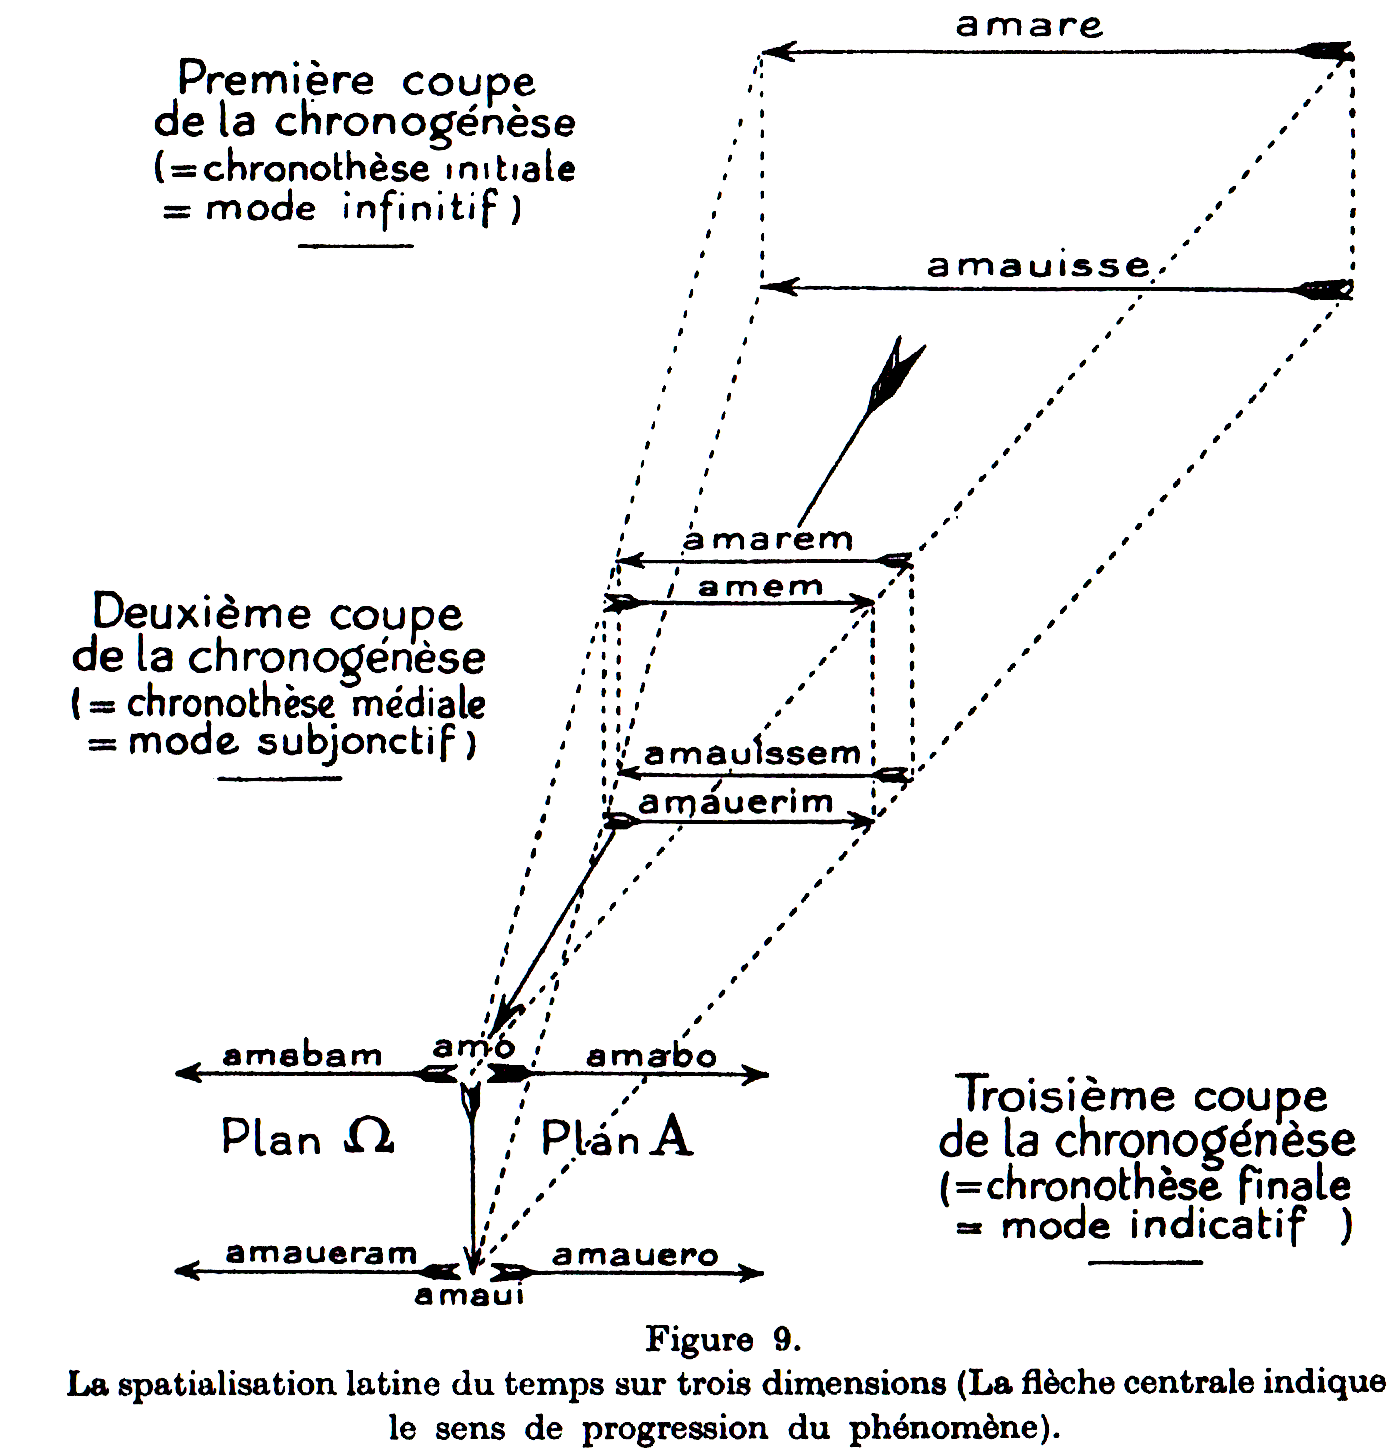
\includegraphics[width=.75\textwidth]{figures/03/Ch3Fig1.png}
\caption{The Latin spatialization of time on three dimensions. From Gustave \citet[37]{guillaume_larchitectonique_1965}.\label{fig:3:1}}
\end{figure}

Guillaume translated his ideas about the relations between time and space into vigorous geometry-like instruments, purportedly reconstructing the mental apparatus of psycholinguistic temporality. According to Guillaume’s diagrams, pre-verbal time comprises \textit{n} dimensions, just like physical space. In this diagram, for example (see \figref{fig:3:1}), Guillaume presented his thesis about the spatial relationships between tenses and moods in Latin. The diagram’s top section shows the infinitive forms: the present infinitive \textit{amāre} (`to love') and below it the perfect infinitive \textit{am{āvisse}}. The central section represents the subjunctive, a binary relationship between two tenses and two aspects: the present and perfect subjunctive (\textit{amem} and \textit{amāverim}), and on top, the same relationship between the anterior actions: the imperfect \textit{amārem} (`I would love to'), and the pluperfect \textit{amāvissem} (`I had loved to'). The lower section of the diagram represents the indicative, the basic form of the verb, with the simple (\textit{amo}) and perfect (\textit{amavi}) forms. The same order relations appear in the past (to the left: the imperfect \textit{amabam} and the pluperfect \textit{amaveram}) and the future (to the right: the future \textit{amabo} and the future perfect \textit{amavero}). The diagram as a whole represents chronogénèse: the mental operation of generating time-images. Each section stands for a chronothèse (initial, medial, and final): the static aspects of the chronogenetical dynamics, fixing the mental time-imagery (\citealt{boone_dictionnaire_1996}).

Guillaume’s inventive terminology, highlighting the dynamic dimension of language, borrowed extensively from physics, geometry, biology and physiology \citep{bottineau_terminologie_2006}. As \citet{valette_conceptualisation_2003} has shown, starting in the 1920s, around the time he expressed his first ideas about psychomechanics, Guillaume gradually adopted more and more scientific terms at the expense of his formerly more richly philosophical vocabulary. The spatialization of time, with its architectonic illustrations and mechanical allure, was the focus of much of Guillaume’s effort to devise an expressly scientific theory of the systematic apparatus underlying language. It allowed Guillaume not only to illustrate the structure of tense systems as he understood it, but also to theorize the cognitive mechanisms motivating grammatical time. In that sense, the spatialization of time, construed here not as a cognitive mechanism but as a strategy of scientification, enabled Guillaume to formulate a proto-science of psycholinguistics.

\section{The conceptual school of cognitive linguistics (1970s to the present)}

By 1975, as similar ideas about the spatial nature of grammatical time were gaining currency among various linguistic schools, the “spatialization of time” was no longer an oddity. “[T]he spatial nature of temporal expressions in many languages is widely recognized,” stated the American linguist Elizabeth C. Traugott in a widely cited article (\citeyear[207]{traugott_spatial_1975}). Inspired by the pioneering works of Eve V. Clark (b. 1942, in \citeyear{clark_acquisition_1971}) and Herbert H. Clark (b. 1940, in \citeyear{moore_space_1973}) on children’s language \is{acquisition}acquisition -- establishing that the same principles that guide general perception determine the acquisition of temporal and spatial vocabulary -- Traugott brought together time-honored diachronic methodologies and novel cognitive sensibilities. Well versed in the writings of Continental \is{structuralists}structuralists, she selected a quote by Guillaume for her article’s epigraph, the same quote I cited above.

Building on existing diachronic datasets, Traugott argued that the grand majority of English \is{prepositions}prepositions derive from locatives, thus demonstrating “[t]he locative character of temporal relations” (\citeyear[209]{traugott_spatial_1975}: 209). Thence, she embarked on ascertaining “whether there are any constraints on the selection of spatial terms for temporal relationships” (\citeyear[207]{traugott_spatial_1975}). This undertaking, attempting to determine the cognitive logic behind the time/space nexus in language, relied on a definition of linguistic time (“the expression of our experience of time”) that Traugott distinguished from both physical and calendrical time (\citeyear[207]{traugott_spatial_1975}). Equipped with a distinct scientific object and a well-defined scientific task, Traugott’s adaptation of the “spatialization of time” theme set an example for future research in the functionalist and cognitive trends. 

Prepositions also attracted the attention of other linguists, such as Leonard Talmy, for whom spatial cognition is a “fine structure”, a fundamental conceptual subdivision of language (\citeyear[225]{pick_how_1983}). Talmy used topological schemata to extrapolate the cognitive principles accounting for the constraints on the distribution of prepositions. Emphasizing the role of spatial cognition in semantics enabled Talmy and other theoretical linguists to connect their work with general cognitive principles, thus linking it to other domains of cognitive science and particularly to research on visual perception and motion. 

For George \citet{lakoff_contemporary_1993} the relations between our notions of time and space are determined by \is{conceptual metaphor}conceptual metaphor. Together with Mark Johnson, he established metaphor as an all-pervasive cognitive mechanism producing concepts and governing semantic change \citep{lakoff_metaphors_1980}. According to their theory of \is{conceptual metaphor}conceptual metaphor (CMT), we conceptualize common abstract concepts, such as \textsc{time}, \textsc{action}, or \textsc{causation} via metaphor, generating non-figurative ideas according to concrete experiences. “Abstract reasoning,” argued Lakoff, “is a special case of image-based reasoning,” mapping mental images from concrete experiential domains onto abstract ones (\citealt[229]{lakoff_contemporary_1993}). Conceptual metaphor builds on visual principles, projecting the structure of one domain onto another, reproducing concepts in new domains, and eventually generating new knowledge. According to Lakoff, the same cognitive mechanisms participate in conceptualizing time: Lacking a biological “detector” of time, we perceive it in terms of objects, locations, and motion in space (\citealt[218]{lakoff_contemporary_1993}).

I employ the term “conceptual school of cognitive linguistics” to refer to those linguists who place concepts and conceptualization at the center of their theoretical work. Cognitive linguists generally portray space not as an abstraction or as a set of cognitive faculties but as a natural concept. Ronald Langacker’s theory, titled \is{Space grammar}\textit{Space grammar} (\citeyear{langacker_space_1982}, \citeyear{langacker_foundations_1987}), is a case in point, treating space as a general conceptual apparatus governing grammatical rationality. For Langacker the priority of space is all-encompassing, applied -- but not limited -- to grammatical temporality. Langacker proposed a particularly elegant specimen of time spatialization when he attempted to provide a semantic construal of lexico-syntactic differences. Hence, the following pair of sentences: 

\ea \label{ex:3:1} The ball curved.
\ex \label{ex:3:2} He threw a curve.
\z
         
exemplify, according to Langacker, two modes of temporal perception governed by a differential visual mechanism (\citeyear[146]{langacker_foundations_1987}, exemple 19). The verbal form in \REF{ex:3:2} expresses \textit{sequential scanning}: a series of event images whose continuous progression replaces one temporal configuration with another. The nominal form in \REF{ex:3:2} stands for a procedure of \textit{summary scanning}: an additive progression of the event image which is accessible simultaneously. While the cognitive modality of sequential scanning simulates a consecutive series of snapshots, during summary scanning snapshots instantly add up to form one visual synthesis. The conceptual difference between conjugated verbs and nominalization, proposes Langacker, is essentially visual: the verbal form expresses the perception of a series of images as a moving sequence (like a motion picture composed of still frames), whereas the noun sums up the complete spatial information in one image. In fact, the semantic difference between the two lexico-syntactic forms reflects the distinction between two general principles underlying spatial cognition and event processing.

As Langacker has explained, the power of space -- both as an epistemic, explanatory principle and as a comprehensive cognitive mechanism governing grammar -- stems from its special status in perception:

\begin{quote}\relax
[I]t hardly seems appropriate or feasible to consider three-dimensional space as a concept definable relative to some other, more fundamental conception. It would appear more promising to regard the conception of space (either two- or three-dimensional) as a basic field of representation grounded in genetically determined physical properties of the human organism and constituting an intrinsic part of our inborn cognitive apparatus. That is, our ability to conceive of spatial relationships presupposes some kind of representational space creating the potential for such relationships, but it is doubtful that conceptual analysis can go beyond positing this representational space and elucidating its properties. (\citealt [148] {langacker_foundations_1987})
\end{quote}

Hence, according to Langacker, space is a primitive concept no other more fundamental idea can ascertain or define. Genetically determined, the conceptual apparatus of space is itself a “representational space,” enabling us to represent spatial relationships. Mirroring its representational competence in a sort of mise-en-abyme, this “representational space” is an innate feature of our cognitive mechanisms grounded in our physiology. This convoluted theory of representation, apparently self-reflecting to infinity, has one clear boundary: the theory’s concept of space begins and ends with the biological necessities constraining the species’ physical and cognitive properties, permitting no further conceptual analysis. 

Cognitive semantics has evolved significantly since the late 1980s, popularizing the idea that linguistic temporality is based on spatial perception. Attempts to advance the thesis of the spatial nature of temporality in language and cognition have often proclaimed subsidiary theoretical goals -- such as ascertaining the universality of temporal experience (e.g. \citealt{alverson_semantics_1994}); advancing a refined research program for linguistic typology (e.g. \citealt{haspelmath_space_1997}); or demonstrating the affinities between language, thought, and cognitive functions such as motor action (\citealt{casasanto_time_2008}). In its various forms, spatialization of time has also served as a more general strategy to enhance grammar’s authority as a scientific form of knowledge.

\section{Conclusion}
Beauzée’s metaphysical tense grammar; Guillaume’s “psychomechanics” of verbal time; late twentieth-century theories about spatial cognition’s role in linguistic temporality -- these three theoretical gestures emerged in very different historical and epistemological contexts. Within these multifaceted contexts the spatialization of grammatical time changed in its foci, forms, and functions. Yet one purpose remained unchanged throughout the centuries: to promote and enhance grammar’s scientification. 

Beauzée was an activist for the cause of the scientification of grammar at a time when the sole established science, in the modern sense, was classical mechanics. Manipulating the similitude between natural and grammatical time, Beauzée conceived his theory of tense with the ambition of changing the course of general grammar. With the example of astronomical physics in mind, Beauzée reconstructed the tense system as a multilayered system of reference, theorizing each tense and the entire tense system as if they were objective constellations, natural phenomena disengaged from discursive considerations. Thus, spatializing time was for Beauzée a strategy for transforming “an old problem,” such as the coherence of the tense system, into “a new science.”

Guillaume’s scientific project developed amid a functioning modern disciplinary environment. However, his interest in the dynamics of psycholinguistic mechanisms ill-fitted the existing framework of normal science, necessitating, in Guillaume’s view, a new scientific language. The idea of time as the fourth dimension of spacetime was then attracting considerable public attention, especially following Einstein’s visit to Paris in~1922 \citep{glick_einsteins_1987}. The growing interest in modern physics most probably also inspired Guillaume’s increasingly science-based terminology. Thus, Guillaume’s “spatialization of time” tied up many loose ends: his interest in the dynamics of verbs and the linguistic expression of time; the need for a psycholinguistic mechanism to associate linguistic temporality with mental images; and the desire to articulate the general laws of language production in a scientific way.

By the 1970s the stakes were very different. The main theoretical concerns of cognitive linguists in the conceptual trend arose within the context of the “Linguistics Wars.” For those hoping to shift linguistic theory’s focus from syntax to semantics, conceptual paradigms like that proposed by the time/space nexus in language came in handy. Space had another significant advantage in the competition between linguistic theories: It linked theoretical linguistics with other fields of cognitive science, enhancing both its empirical and its theoretical standing. Spatializing time allowed cognitive semantics to demonstrate how general principles of cognition propose semantic explanations while reshuffling traditional distinctions like that between lexicon and grammar. 

There is wide agreement among historians of linguistics as to the high degree of continuity in the history of linguistic ideas and the discipline’s low “rewriting rate” (\textit{taux de réinscription}) -- a concept Sylvain \citet{auroux_histoire_1980} introduced to emphasize that linguistics progresses without eradicating past theories via paradigmatic change. The continuity traced in this study is not historical per se: it is difficult to measure the degree of influence Beauzée’s work had on Guillaume’s “spatialization of time,” and Traugott’s reference to Guillaume was clearly superficial. Yet, I would like to argue that this genealogical study of the spatialization of grammatical time suggests that the history of scientificity \citep{auroux_techne_1990} and scientification cannot solely rely on isolated evidence documenting the transmission of knowledge by individuals. It must also be attentive to scientific motivations and to the concrete webs of interests wherein these motivations are situated. Such a theoretical framework could enrich our understanding of the modes of continuity and progression typical of linguistics and the way it functions as a scientific discipline. This study of time spatialization shows that, whenever the modern concept of space was available to them, linguists employed the novel practices and opportunities it opened up to promote the scientification of grammar. Understood as a strategy, spatialization of time may illuminate the ways by which scientific memory persists and prevails.

% % \section*{Acknowledgements}

{\sloppy\printbibliography[heading=subbibliography,notkeyword=this]}
\end{document}
